\documentclass[aspectratio=169]{beamer}
%\documentclass{beamer}
\beamertemplatenavigationsymbolsempty
\usecolortheme{beaver}
\setbeamertemplate{blocks}[rounded=true, shadow=true]
\setbeamertemplate{footline}[page number]
%
\usepackage[utf8]{inputenc}
\usepackage[english,russian]{babel}
\usepackage{amssymb,amsfonts,amsmath,mathtext}
\usepackage{subfig}
\usepackage[all]{xy} % xy package for diagrams
\usepackage{array}
\usepackage{bm}
\usepackage{multicol}% many columns in slide
\usepackage{hyperref}% urls
\usepackage{hhline}%tables
\usepackage{mathtools}
\usepackage{graphicx}
\captionsetup[subfigure]{font={small},labelfont={small}}
\usepackage{adjustbox}
% Your figures are here:
\graphicspath{ {fig/} {../fig/} }
\newtheorem{theorem_rus}{Теорема}
\newtheorem{lemma_rus}{Лемма}
\setbeamertemplate{theorems}[numbered]
\setbeamertemplate{caption}[numbered]
\usepackage{ragged2e}
\usepackage[T1]{fontenc} % Кодировка шрифтов для западных языков
\usepackage[utf8]{inputenc} % Кодировка UTF-8
\usepackage[english]{babel} % Поддержка английского языка

\usepackage[style=authoryear,language=english]{biblatex}
\addbibresource{references.bib} % Файл с библиографией
\justifying
% latin bold lower
\newcommand{\ba}{\mathbf{a}} 
\newcommand{\bc}{\mathbf{c}} 
\newcommand{\be}{\mathbf{e}} 
\newcommand{\bh}{\mathbf{h}} 
\newcommand{\bp}{\mathbf{p}} 
\newcommand{\bt}{\mathbf{t}} 
\newcommand{\bs}{\mathbf{s}} 
\newcommand{\bu}{\mathbf{u}} 
\newcommand{\bv}{\mathbf{v}} 
\newcommand{\bw}{\mathbf{w}} 
\newcommand{\bx}{\mathbf{x}} 
\newcommand{\by}{\mathbf{y}} 
\newcommand{\bz}{\mathbf{z}} 

% latin bold upper
\newcommand{\bA}{\mathbf{A}} 
\newcommand{\bB}{\mathbf{B}} 
\newcommand{\bC}{\mathbf{C}} 
\newcommand{\bI}{\mathbf{I}} 
\newcommand{\bJ}{\mathbf{J}} 
\newcommand{\bL}{\mathbf{L}} 
\newcommand{\bM}{\mathbf{M}} 
\newcommand{\bP}{\mathbf{P}}
\newcommand{\bQ}{\mathbf{Q}} 
\newcommand{\bR}{\mathbf{R}} 
\newcommand{\bT}{\mathbf{T}} 
\newcommand{\bU}{\mathbf{U}} 
\newcommand{\bV}{\mathbf{V}} 
\newcommand{\bW}{\mathbf{W}} 
\newcommand{\bX}{\mathbf{X}} 
\newcommand{\bY}{\mathbf{Y}} 
\newcommand{\bZ}{\mathbf{Z}} 

% latin cal upper
\newcommand{\cF}{\mathcal{F}} 
\newcommand{\cG}{\mathcal{G}} 
\newcommand{\cI}{\mathcal{I}} 
\newcommand{\cL}{\mathcal{L}} 
\newcommand{\cM}{\mathcal{M}} 
\newcommand{\cN}{\mathcal{N}} 
\newcommand{\cS}{\mathcal{S}} 
\newcommand{\cT}{\mathcal{T}} 
\newcommand{\cW}{\mathcal{W}} 
\newcommand{\cX}{\mathcal{X}} 
\newcommand{\cZ}{\mathcal{Z}} 

% latin bb upper
\newcommand{\bbE}{\mathbb{E}} 
\newcommand{\bbI}{\mathbb{I}} 
\newcommand{\bbP}{\mathbb{P}} 
\newcommand{\bbR}{\mathbb{R}}
\newcommand{\bbX}{\mathbb{X}} 
\newcommand{\bbY}{\mathbb{Y}}
\newcommand{\bbW}{\mathbb{W}} 

% greek bold lower
\newcommand{\bepsilon}{\boldsymbol{\epsilon}} 
\newcommand{\btheta}{\boldsymbol{\theta}} 
\newcommand{\blambda}{\boldsymbol{\lambda}} 
\newcommand{\bpi}{\boldsymbol{\pi}} 
\newcommand{\bmu}{\boldsymbol{\mu}} 
\newcommand{\bsigma}{\boldsymbol{\sigma}} 
\newcommand{\bphi}{\boldsymbol{\phi}} 

% greek bold upper
\newcommand{\bSigma}{\boldsymbol{\Sigma}} 

\DeclareMathOperator*{\argmin}{arg\,min}
\DeclareMathOperator*{\argmax}{arg\,max}

% transpose
\newcommand{\T}{^{\text{\tiny\sffamily\upshape\mdseries T}}}


\newcommand{\bb}{\mathbf{b}}
\newcommand{\bq}{\mathbf{q}}
\newcommand{\bS}{\mathbf{S}}
\newcommand{\bH}{\mathbf{H}}

\newcommand{\bE}{\mathbf{E}}
\newcommand{\bF}{\mathbf{F}}
\newcommand{\bomega}{\boldsymbol{\omega}}

\newcommand{\bgamma}{\boldsymbol{\gamma}}
\newcommand{\bdelta}{\boldsymbol{\delta}}
\newcommand{\bPsi}{\boldsymbol{\Psi}}
\newcommand{\bpsi}{\boldsymbol{\psi}}
\newcommand{\bxi}{\boldsymbol{\xi}}
\newcommand{\bchi}{\boldsymbol{\chi}}
\newcommand{\bzeta}{\boldsymbol{\zeta}}
\newcommand{\beps}{\boldsymbol{\varepsilon}}
\newcommand{\bZeta}{\boldsymbol{Z}}
% mathcal

\newcommand{\cY}{\mathcal{Y}}
\newcommand{\dH}{\mathds{H}}
\newcommand{\dR}{\mathds{R}}
%----------------------------------------------------------------------------------------------------------
\title[\hbox to 56mm{Краткое название}]{Robust Detection of AI-Generated Images}
\author[Д.\,Д.~Дорин]{Даниил Дмитриевич Дорин\\
\small Научный руководитель: к.ф.-м.н. А.\,В.~Грабовой \\
\small Ассистент: Д.\,Д.~Дорин}
\institute{Анализ данных ФПМИ МФТИ}
\date{2025}

%----------------------------------------------------------------------------------------------------------
\begin{document}
%----------------------------------------------------------------------------------------------------------
\begin{frame}
\thispagestyle{empty}
\maketitle
\end{frame}

%----------------------------------------------------------------------------------------------------------
\begin{frame}{Цель и постановка задачи}
\begin{block}{Цель работы}
    Построить модель классификации изображений на сгенерированные и реальные, устойчивую к методам генерации. 
\end{block}
\begin{block}{Постановка задачи}
Задана выборка $$\mathfrak{D} = \{\mathbf{x_i}, y_i \},\ i= 1, ..., N,$$ где $\mathbf{x_i} \in \mathbb{N}^{m \times n \times r}$ - изображение разрешения $m \times n$ с  $r$ каналами, $y_i \in \{ 0, 1\}$ \\

Строится отображение $\mathbf{F}: \mathbb{N}^{m \times n \times r} \rightarrow [0, 1] $ - отображение из изображения в вероятность того, что изображение сгенерированно.

Решается задача нахождения оптимального отображения \( \mathbf{F}^* \) в своём классе моделей \( \mathcal{F} \), т.е.:
\[
	\mathbf{F}^* = \arg\min_{\mathbf{F}^* \in \mathcal{F}} \operatorname{Log Loss}(F).
\]
\end{block}
\end{frame}
%----------------------------------------------------------------------------------------------------------
\begin{frame}{Ошибки на моделях, качество классификатора}
\begin{figure}
\centering
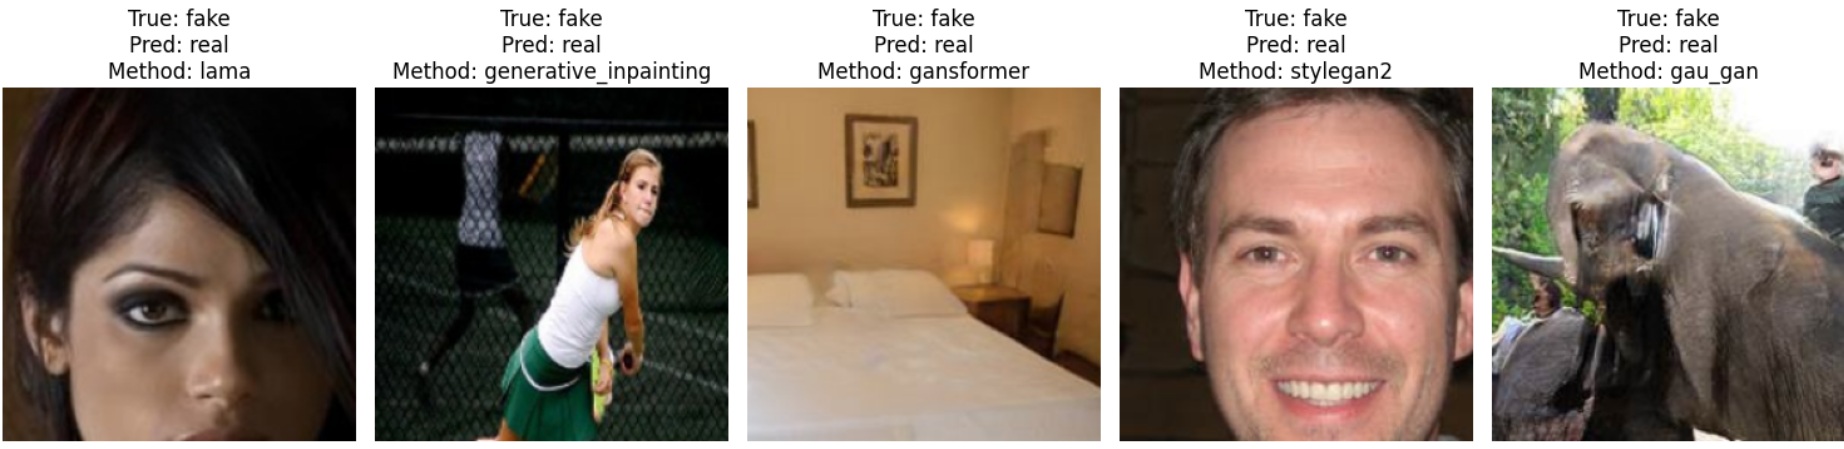
\includegraphics[width=0.76\textwidth]{figs/fake_images.png}
\end{figure}

\begin{figure}
\centering
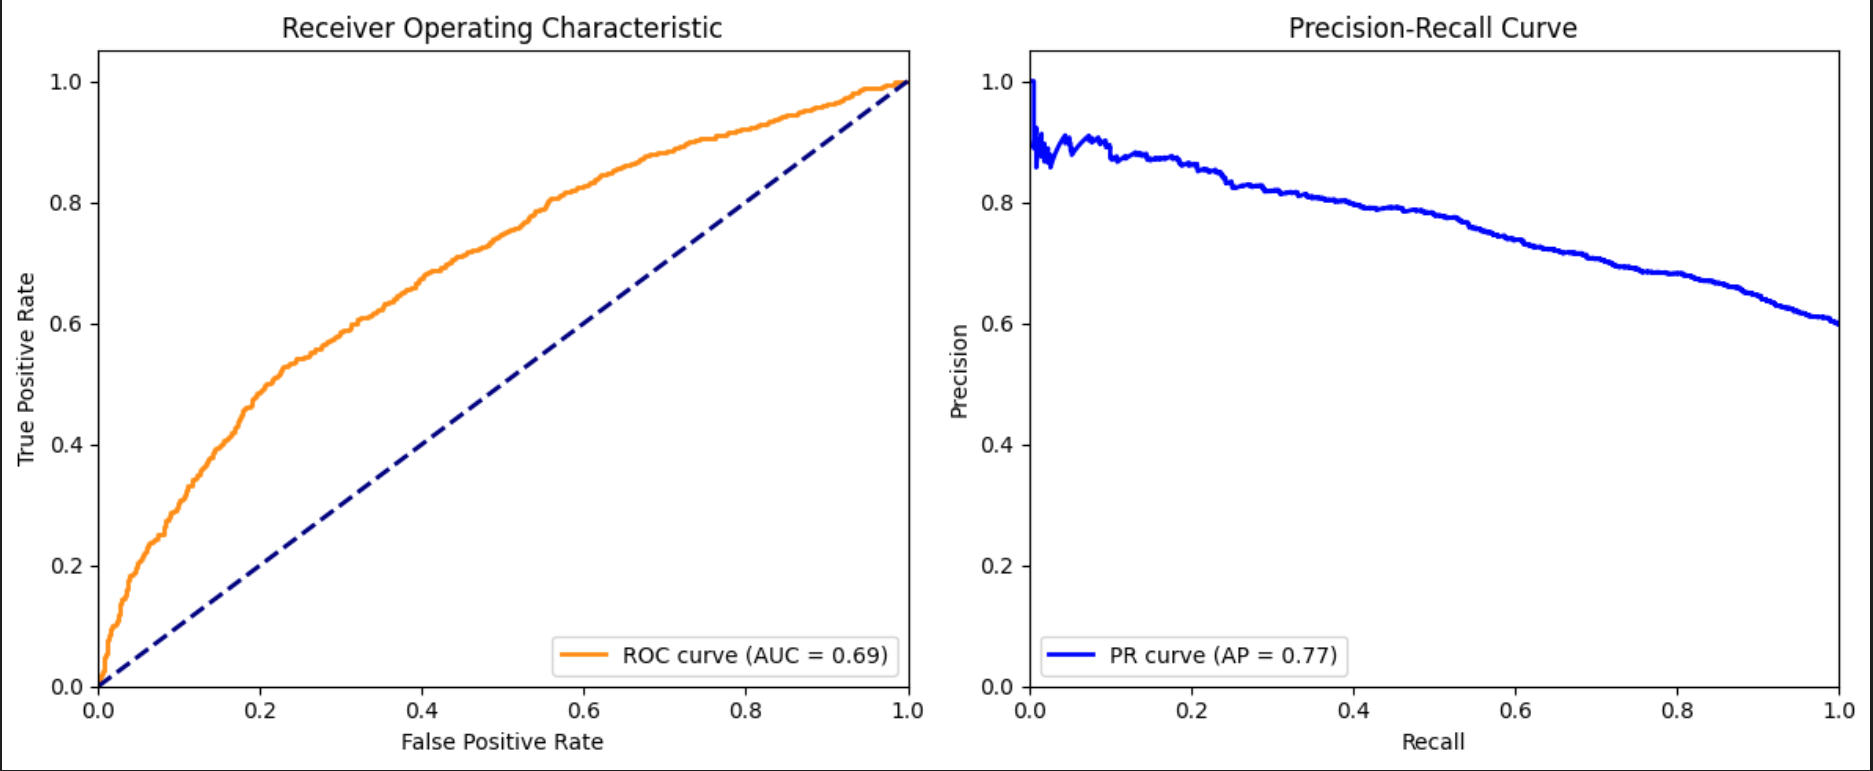
\includegraphics[width=0.66\textwidth]{figs/PR_ROC.png}
\end{figure}
\end{frame}
%----------------------------------------------------------------------------------------------------------
\end{document} 